\documentclass{article}
\usepackage[utf8]{inputenc}
\newcommand{\ii}{{\bf i}}
\newcommand{\jj}{{\bf j}}
\newcommand{\kk}{{\bf k}}
\newcommand{\id}{{\bf 1}}
\newcommand{\hur}{\frac{\id+\ii+\jj+\kk}{2}}%The "Hurwitz point"
\newcommand{\hurwitz}{\Z\left[\hur,\ii,\jj,\kk\right]}%The set of Hurwitz integers
\usepackage{wrapfig}
\usepackage[utf8]{inputenc}
\usepackage[dvips]{graphicx}
\usepackage{a4wide}
\usepackage{amsmath}
\usepackage{euscript}
\usepackage{amssymb}
\usepackage{amsthm}
\usepackage{amsopn}
\usepackage[colorinlistoftodos]{todonotes}
\usepackage{graphicx}
\usepackage[T1]{fontenc}
\newcommand\mybar{\kern1pt\rule[-\dp\strutbox]{.8pt}{\baselineskip}\kern1pt}

\usepackage{ulem}
\usepackage{xcolor}
\newcommand{\cs}[1]{\color{blue}{#1}\normalcolor}

%Matrix commands
\newcommand{\ba}{\begin{array}}
\newcommand{\ea}{\end{array}}
\newcommand{\bmat}{\left[\begin{array}}
\newcommand{\emat}{\end{array}\right]}
\newcommand{\bdet}{\left|\begin{array}}
\newcommand{\edet}{\end{array}\right|}

%Environment commands
\newcommand{\be}{\begin{enumerate}}
\newcommand{\ee}{\end{enumerate}}
\newcommand{\bi}{\begin{itemize}}
\newcommand{\ei}{\end{itemize}}
\newcommand{\bt}{\begin{thm}}
\newcommand{\et}{\end{thm}}
\newcommand{\bp}{\begin{proof}}
\newcommand{\ep}{\end{proof}}
\newcommand{\bprop}{\begin{prop}}
\newcommand{\eprop}{\end{prop}}
\newcommand{\bl}{\begin{lemma}}
\newcommand{\el}{\end{lemma}}
\newcommand{\bc}{\begin{cor}}
\newcommand{\ec}{\end{cor}}
\newcommand{\lcm}{\mbox{lcm}}
\newcommand{\defn}{\fbox{definition}}
\newcommand{\prop}{\fbox{proposition}}
\newcommand{\stab}{\mbox{stab}}



%sets of numbers
\newcommand{\N}{\mathbb{N}}
\newcommand{\Z}{\mathbb{Z}}
\newcommand{\Q}{\mathbb{Q}}
\newcommand{\R}{\mathbb{R}}

\title{Abstract Algebra}
\author{August, Evelyn}
\date{10/05/2021}

\begin{document}
\maketitle
\fbox{32, question} If $\beta = (14523)$, what is $\beta^{99}$.\\
\fbox{answer} One possible approach would be to compute this directly. But this would not be fun, and is probably better left for python or some other programming language. Instead, let's use a better method.\\
First, note that by theorem 5.3 $|\beta| = 5$, as the least common multiple of the length of the only disjoint cycle used to represent $\beta$ is just the length of the cycle used to represent $\beta$. By the associative property of groups and the definition of order, and since $\beta\in S_5$ which is a group, it follows that $\beta^{99} = (\beta^5)^{19}\beta^4 = \epsilon\beta^4 = \beta^4 = (\beta^2)^2$. So we want to find $\beta^2$. To do this, we simply compose $(\beta\circ \beta = (14523))(14523) = (15342).$ Substituting, $\beta^4 = (\beta^2)^2 = (15342)(15342) = (13254)$. Hence $\beta^{99} = (13254)$.\\

\fbox{alternatively} Someone pointed out that I copied the problem down wrong, and that we were originally given that $\beta = (123)(145)$. In this case, since $4\equiv -1\pmod{5 = |\beta|}$, it follows that $\beta^{99} = \beta^{-1}$. If we reverse the order of the cycles with which $\beta$ is written as well as the order of the entries within the cycles, we have $(154)(132)=(13254)=\beta^{-1}=\beta^{99}$.

\fbox{35, proposition} Let $G$ be a group of permutations on a set $X$ and let $\stab(a) = \{\alpha\in G : \alpha(a) = a, \forall a\in G\}$. Then $\stab(a)\le X$.\\

\fbox{proof} Let $G,X$ be instantiated as stated in the proposition, and let $a\in X$ be an arbitrary element in $X$. Since $G$ is a subgroup of permutations, $G$ cannot be empty. We just need to show closure and the existence of inverses for all elements in stab(a). Thus, first we want to prove that for all elements $\alpha,\beta\in \stab(a)$, $\alpha\beta \in \stab(a)$. By definition of $\stab(a)$ and function composition, $\alpha\circ \beta (a)  = \alpha(\beta(a)) = \alpha(a) = a$. Hence $\alpha\beta\in \stab(a)$.\\

Let $\alpha$ be an arbitrary element in $\stab(a)$ Since $G$ is a group of permutations, and since $\stab(a)\subseteq G$, there exists some $\alpha^{-1} \in G$ such that $\alpha\circ\alpha^{-1} = \epsilon = \alpha^{-1}\circ \alpha$. Let $a\in G$ be arbitrary. Then by composition, $\alpha\circ\alpha^{-1}(a) = \alpha(\alpha^{-1}(a)) = \alpha^{-1}(a)=a$. Thus, it follows that $a^{-1}\in$ stab(a) for all $a \in$ stab(a), hence $\stab(a)$ satisfies the inverse property.\\


\fbox{43, question} What is are some example of element $\alpha,\beta\in S_5$ where $|\alpha| = 3 = |\beta|$ and $|\alpha\beta| = 5$.\\
\fbox{answer} Try $(123)$ and $(345)$. Composing, $(123)(345) = (12345)$ By theorem 5.3, $|(123)| = |(123)| = 3$ and $|(12345)| = 5$. Furthermore, since these are permutations of 5 same elements, all of these elements are in $S_5$.\\

\fbox{lemma} A cycle of even length is odd, and a cyclic of odd length is even. Furthermore, the product of an even cycle and an odd one is an odd cycle, and the product of two cycles of the same parity is even.\\
\fbox{proof} Let $\alpha = (a_1,\dots,a_n)$ be a cycle for some even $n\in \N$. Consider the permutation $\beta = [\beta_1=(a_1a+2)]\dots[\beta_n = (a_1a_n)]$. $\beta$ is even, as there it is represented here as a product of an even number of two cycles. It remains to be shown that $\alpha = \beta$. Then $\alpha(a_1) = a_2$ and $\beta(a_1) = \beta_1(\beta_2(\dots\beta_n(a_1))\dots).$

\fbox{61, proposition} There are 24 elements in $A_5$ of order $5$, $20$ elements of order $3$ and $15$ of order $2$.\\

\fbox{proof} Writing out the possible combinations of disjoint cycles in $S_5$, we have 

$$
\begin{array}{cc}
     a&  (\underline{5})\\
    b & (\underline{4})(\underline{1})\\
    c & (\underline{3})(\underline{2})\\
    d & (\underline{3})(\underline{1})(\underline{1})\\
    e & (\underline{2})(\underline{1})(\underline{1})(\underline{1})\\
    f & (\underline{2})(\underline{2})(\underline{1})\\
    g & (\underline{1})(\underline{1})(\underline{1})(\underline{1})(\underline{1}).
\end{array}
$$
By theorem 5.5, only cycles in forms a,d, f, and g are even. By Ruffini's theorem, cycles of form a have order 5, d of order 3, and f of order 2. Furthermore, for the number of elements of form a, we have $5!/5 = 24$ possible elements (this is because we are permuting 5 elements in five slots, but don't care about rotations). For elements of order 3 we have $5!/(2\cdot 3)=20$, since we are again permuting 5 elements, however, we do not care about the rotations in the 3-cycle as well as switching the position of the two 1-cycles. And for elements of order 2 we have $5!/(3!\cdot 2) \cdot 3!/(2\cdot 2)=15$ possible elements, since we have $\binom{5}{2}$ options for filling the first 2-cycle and $\binom{3}{2}$ options for filling the second 2-cycle. Since we do not care about the arrangement of the two 2-cycles we divide it once more by 2. Hence, we see that we have 24 elements in $A_5$ of order 5, 20 elements of order 3 and 15 of order 2. 
\\
\fbox{81, problem}

Show how these arrangements are permutations in $S_4$.
\begin{figure}[htbp]
\centerline{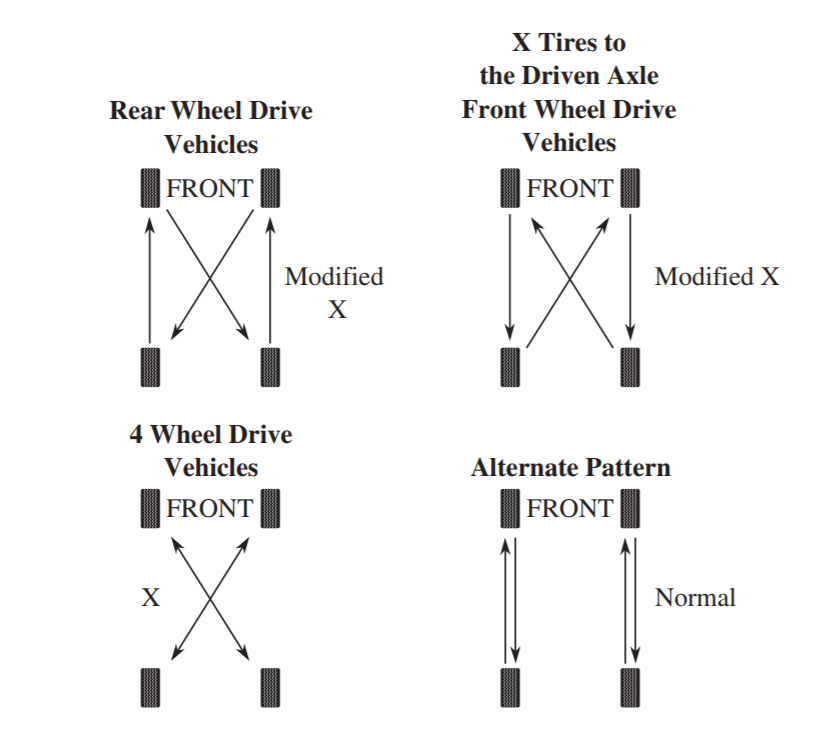
\includegraphics[scale=0.5]{tires1.png}}
\caption{tire arrangements}
\label{fig}
\end{figure}
First, number the tires as such
\begin{figure}[htbp]
\centerline{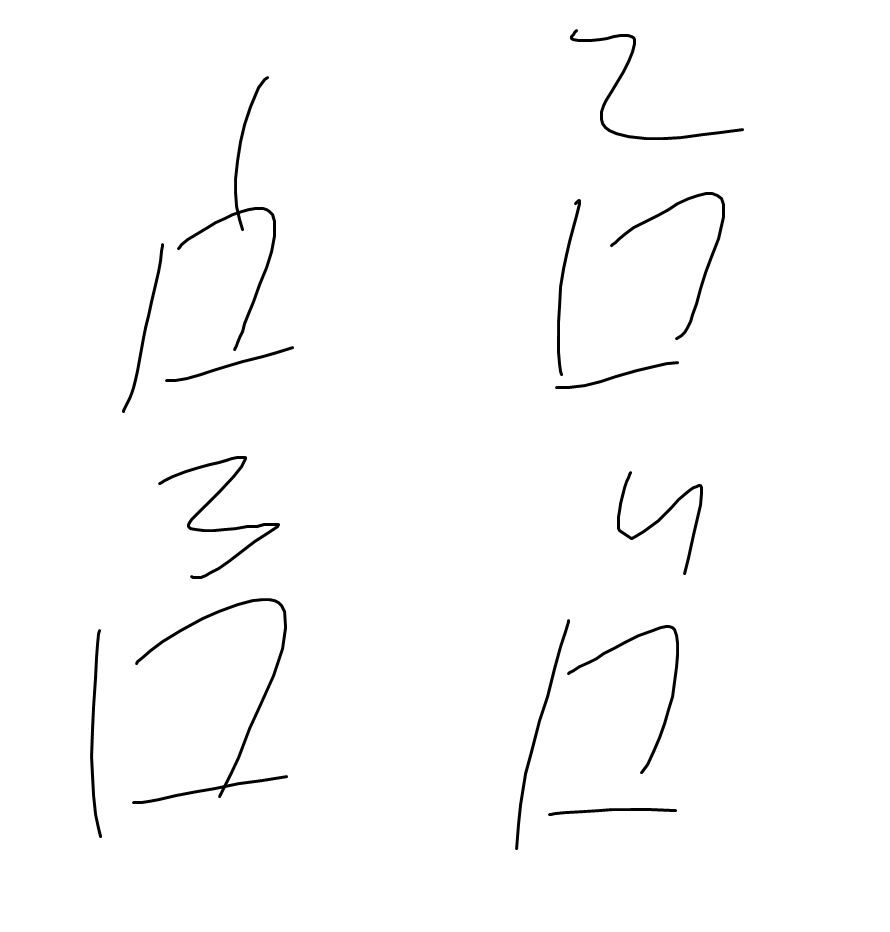
\includegraphics[scale=0.1]{tires.png}}
\caption{numbering}
\label{fig}
\end{figure}
Then the top-left arrangement can be described as a permutation that sends 1 to 4, 4 to 2, 2 to 3, and 3 back to 1. In cyclic notation, the top-left arrangement can be written $\alpha = (1423)$. Likewise, the top-right can be written $\beta = (1324)$, the bottom left $\gamma = (14)(23)$, and the bottom right $\kappa = (13)(24)$. For convenience, call the set of these four permutations $T$. \\

Clearly $T$ is not a subgroup of $S_4$, as it is not a group under function composition. There is no identity element. Nor is it closed. Take for example the composition $\gamma\kappa = (14)(23)(13)(24) = (12)(34) = \sigma$. Clearly this is not an element of $T$. \\


\fbox{solution} For extra clarity, I will re-list each of the elements of $T$: $\alpha = (1423), \beta = (1324), \gamma = (14)(23), \kappa = (13)(24)$. Furthermore, we have $\kappa\gamma = (13)(24)(14)(23) = (12)(34) = \sigma$. Also $\alpha\beta = \epsilon$, where $\epsilon$ is the identity permutation. Also, $\alpha\gamma = (12) = \nu$, $\aplha^2 = (12)(34) = \sigma$. We keep doing this until we get a list of eight elements,
$$\begin{array}{cc}
     &  \epsilon = (1)\\
&\alpha = (1423)\\
&\beta = (1324)\\
&\gamma = (14)(23)\\
&\kappa = (13)(24)\\
&\sigma = (12)(34)\\
&\mu = (34)\\
&\nu= (12)\\
\end{array}.$$
Drawing out a cayley table (these start to fill themselves in after a while once we can substitute and use associativity for our convenience), we have this \\

\begin{wrapfigure}{0.5\textwidth}

    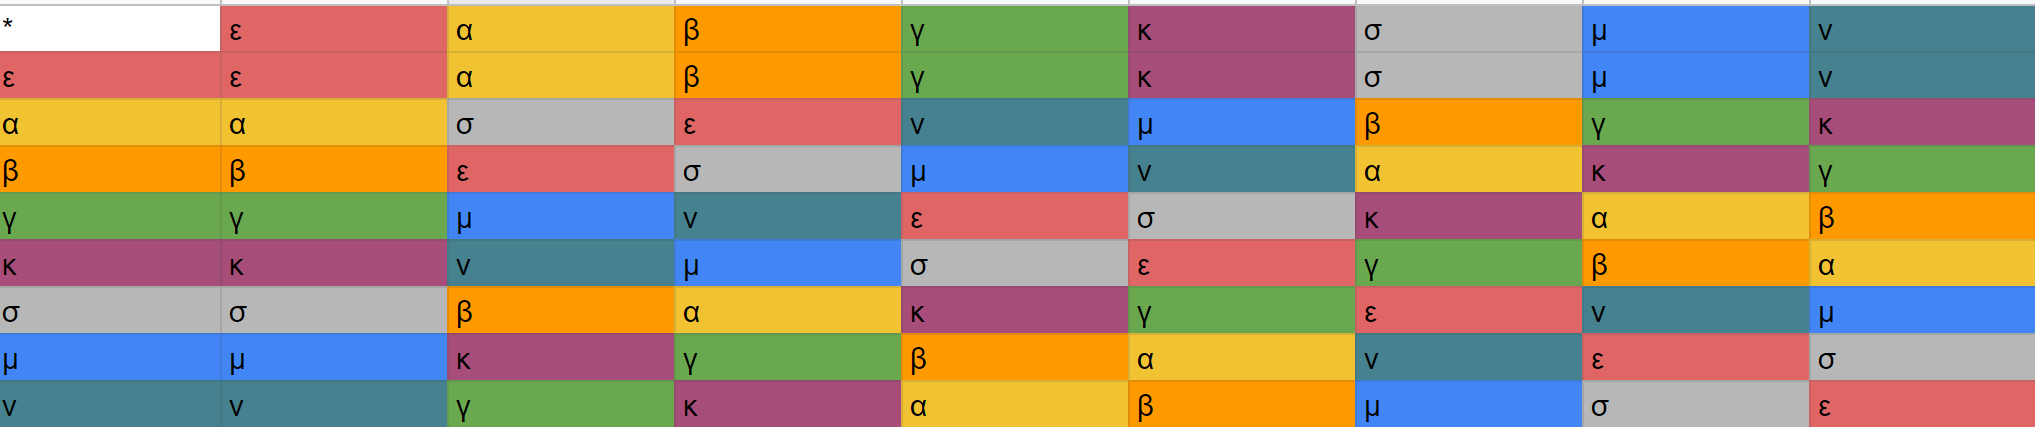
\includegraphics[width=1\textwidth]{cayley table.png}
  \caption{cayey table}
\end{wrapfigure}
\\

Thus, by analyzing the cayley table we notice that the set S containing the permutations $\alpha, \beta, \gamma, \kappa, \sigma, \mu, \nu$, and $\epsilon$ forms a group under function composition, since we have the identity element $\epsilon$, every element in the group has an inverse and the group is closed under its operation. Additionally, we see that the group is not Abelian. \\

\end{document}